
\phChapterWorksheet{Go Get All of 'em!}{Find where the \mappMobimon{} are running loose}

While catching \mappMobimon{} on \textbf{Road 2,} you run across a wise old
\mappMobimon{} trainer who challenges you to a \mappMobimon{} battle. But not
just any \mappMobimon{} battle! This is a \textbf{puzzle battle.} The reward?
The location where all the \mappMobimon{} gather.

The old man tells you about a game he enjoyed in his youth called \textbf{Go.}

Go is a game of strategy played with black and white pieces on a grid. It's a
bit like chess, except instead of lots of kinds of pieces, each player only has
\textbf{one kind of piece, the stone.} And instead of playing on the squares,
players play on the \textbf{intersections of the grid lines,} and you can play
on board going from 9 by 9 up to 19 by 19. And \textbf{black goes first.} Maybe
it's not all that much like chess.

Much like chess, though, part of the strategy relies on \textbf{capturing your
  opponent's stones.} To capture you have to know about stones, groups of
stones, and their \textbf{liberties.}

Stones typically don't stay isolated for very long from other stones of the same
color. Stones form a \textbf{group} if they are \textbf{directly next to each
  other on the grid,} but \textbf{not diagonally.}

\gobansize{9}
These stones form a group.

\black{b2,c2,d2}
\begin{center}
  \showgoban
\end{center}
\cleargoban

These stones \textbf{do not.} These are just three individual stones.

\black{b2,c3,d4}
\begin{center}
  \showgoban
\end{center}
\cleargoban

An individual stone has \textbf{liberties.} Liberties are the \textbf{empty
  spaces directly next to the stone on the grid,} but \textbf{not diagonally.}
So a stone may have \textbf{as many as 4} liberties. If an individual stone has
no liberties, \textbf{it is captured.}

The liberties of the black stones are marked with x's:

\black{b2,d4}
\white{e4,d5}
\gobansymbol{b1,b3,a2,c2,c4,d3}{x}
\begin{center}
  \showgoban
\end{center}
\cleargoban
\cleargobansymbols

So the black stone on the lower left has \textbf{4 liberties,} and the black
stone on the upper right \textbf{only has two liberties} because the other two
spaces around it are occupied by white stones.

\textbf{Groups of stones share liberties.} A whole group of stones can be
captured at the same time if the whole group has no liberties. The group of
black stones below has \textbf{7 liberties.}

\black{b2,c2,c3}
\gobansymbol{b1,a2,b3,c4,d3,d2,c1}{x}
\begin{center}
  \showgoban
\end{center}
\cleargoban
\cleargobansymbols

A stone can normally \textbf{not} be played in a space where it has no
liberties, with \textbf{one important exception.} A stone can be placed into a
space where it would have no liberties only if doing so \textbf{captures one or
  more enemy stones.}

The old man lays out several boards in an intermediate size, then says, ``In
each of the Go boards below, there is exactly one stone you can play, white or
black, that will allow you to make a capture. You need to figure out
\textbf{what color stone} to play and \textbf{where to play it} in order to make
a capture. Do that, and you will already know where all the \mappMobimon{}
gather.''

You notice that each of the boards the old man shows you is \textbf{13 by
  13.} There are also \textbf{26 letters in the alphabet.} Hmmm...

\gobansize{13}

\white{f4,g3,g5,h4}
\black{h3,h5,j4}
\begin{center}
  \showfullgoban
\end{center}

\cleargoban
\white{c7,d8,e7,e8,e9,f9}
\black{c6,d5,d7,e5,e6}
\begin{center}
  \showfullgoban
\end{center}

\cleargoban
\white{k9,l9,m5,m7,m8,m11,n7,n11}
\black{l10,m9,m10,n4,n5,n8,n10}
\begin{center}
  \showfullgoban
\end{center}

\cleargoban
\white{a6,b7,b9,b10,c10,d7,d10,e8,e9,f9}
\black{a7,a8,c9,d8,d9,e6,e7}
\begin{center}
  \showfullgoban
\end{center}

\cleargoban
\white{a8,b7,c6,c9,d5,d8,e5,e7,f6}
\black{b8,c7,c8,d6,d7,e6}
\begin{center}
  \showfullgoban
\end{center}

\cleargoban
\white{a11,b11,c11,c12,c13}
\black{a10,a12,b10,b13,c10,d10,d11,d12,d13}
\begin{center}
  \showfullgoban
\end{center}

\cleargoban
\white{b7,b10,c7,c8,c11,c12,c13,d9,e8,e10,f9,g7,h7}
\black{a8,c9,c10,d8,d10,d11,e7,e11,f6,f7,f8,f10,g9,g10}
\begin{center}
  \showfullgoban
\end{center}

\cleargoban
\white{c10,d7,e9,e10,f8,f10,g8,h7,h8,j8,k5,k8,k9}
\black{c11,e8,f9,g7,g9,h6,h9,j5,j6,j7,j9,k4,k7,k10,l8,l9,m9}
\begin{center}
  \showfullgoban
\end{center}

\cleargoban
\white{g7,g8}
\black{e5,f3,f4,f7,f8,g3,g6,h2,h7,h8,j2,k2,k7,k8,l3,l6,l9,m3,m4,m7,m8,n5}
\begin{center}
  \showfullgoban
\end{center}

\cleargoban

Where should you find the \mappMobimon{}?

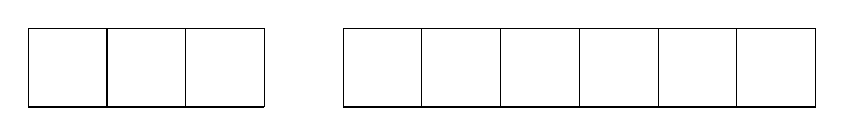
\begin{tikzpicture}
  \draw (0,0) grid (3,1);
  \draw (4,0) grid (10,1);
\end{tikzpicture}

% Include below for aucTeX integration
%%% Local Variables:
%%% mode: latex
%%% TeX-master: "../mapp-challenge-18-game-book"
%%% End:
